\documentclass{article}
\usepackage{iclr2027_conference,times}
\usepackage[T1]{fontenc}
\usepackage{amsmath,amssymb,booktabs,tabularx,microtype}
\usepackage{float}
\usepackage{hyperref}
\usepackage{url}
\hypersetup{hidelinks}
\usepackage[section]{placeins}
\usepackage{tikz}
\usetikzlibrary{arrows.meta,positioning}
\setlength{\emergencystretch}{2em}
\title{CoSpRo: Concept-Guided\\Relational Pretraining for\\Spurious-Correlation Robustness}
\author{}
\begin{document}
\maketitle
\begin{abstract}
Self-supervised representations can inherit spurious object--context associations from unlabeled images. We introduce CoSpRo, a method that uses sparse, language-aligned concepts to discover relations for more robust representation learning. A frozen CLIP/SpLiCE teacher identifies image pairs that become more similar after selected concept subspaces are removed. Activation contrast, residual concept agreement and synthetic null controls filter these relations into a sparse weighted graph. The graph guides batch composition and a relational objective alongside ordinary SimCLR, without target or group annotations during pretraining. Only the student encoder is needed at inference. A four-seed Waterbirds study yields higher mean worst-group accuracy than SimCLR and budget-matched raw-CLIP graph supervision. Semantic-neighbour and direct-transfer controls help separate the role of projected relations from the information in the frozen representation, while exposing uncertainty in the gains and imperfect preservation of target semantics.
\end{abstract}

\section{Introduction}
An image can contain several predictive factors. In Waterbirds, bird category correlates with background in the training set. A representation that strongly encodes this association can fail on birds shown in an uncommon environment. Worst-group evaluation makes these failures visible even when aggregate accuracy appears acceptable \citep{sagawa2020groupdro}. Self-supervised pretraining inherits the correlations present in its unlabeled images. Standard view augmentation alone does not specify which context changes should preserve object identity.

Our goal is to learn a visual encoder whose downstream predictions remain useful when object--context associations change, using no target labels or group annotations during graph construction and representation learning. A frozen vision-language model supplies semantic structure learned from external data. SpLiCE exposes this structure as sparse non-negative coordinates associated with text concepts \citep{bhalla2024splice}. We hypothesize that a concept subspace can explain why two images appear dissimilar. Removing that subspace may reveal a useful relation for student training. Those concepts can also encode object identity and projection can introduce incorrect downstream classifications.

CoSpRo constructs a fixed teacher graph from projected relations. Each candidate relation is evaluated using geometric gain, concept activation contrast and agreement in the remaining sparse coordinates. Synthetic nulls calibrate group selection. The graph determines batch composition and supplies soft relational targets on the student backbone. During inference only the trained encoder and downstream classifier are required.

Our contribution is a concept-projected relation-discovery method and a controlled study of its transfer to an independently trained encoder. The graph exposes which concept removal produced each retained relation. The experimental design separates this choice of neighbours from graph-aware sampling and generic CLIP supervision. The four-seed study tests student transfer alongside graph quality and direct prediction of frozen SpLiCE representations.

\section{Related Work}
\paragraph{Selecting examples and relations in contrastive learning.}
SimCLR contrasts two views of an image against other images in the batch \citep{chen2020simclr}, making sample selection part of the learning signal. Hard-negative sampling emphasizes examples that are difficult to distinguish from an anchor without requiring labels \citep{robinson2021hard}. Debiased contrastive learning corrects contamination by same-class negatives \citep{chuang2020debiased}; false-negative cancellation instead identifies likely semantic matches for elimination or attraction \citep{huynh2022false}. NNCLR explicitly uses nearest neighbours as cross-image positives \citep{dwibedi2021nnclr}. CoSpRo also changes which images meet in a batch, but retains within-image SimCLR positives and all other images in its negative denominator. A separate backbone loss transfers the graph relations.

\paragraph{Constructing informative batches.}
Batch construction has been studied as a way to change the in-batch contrastive signal. GCBS globally arranges examples so that informative pairs fall within batches \citep{sachidananda2023gcbs}. BatchSampler samples batches by random walks on a proximity graph, balancing hard negatives against false-negative contamination \citep{yang2023batchsampler}. B3 builds a sparse graph from pretrained teacher rankings and samples graph communities to obtain strong in-batch negatives \citep{thirukovalluru2025b3}. Concept-Aware Batch Sampling instead selects image--text training examples to control concept diversity or frequency within a batch \citep{ghosh2026cabs}. Language-guided visual learning uses caption similarity to choose cross-image positive pairs \citep{elbanani2023language}. CoSpRo pretraining stage builds a fixed relation graph, which both influences sample batching and supplies soft targets through a separate backbone loss. Cross-image graph neighbours still remain negatives in the SimCLR, even though images with high similarity are more likely to appear in the same batch during student training. The sampler-only ablation is provided to test whether co-location alone helps in downstream task.

\paragraph{Concept representations, discovery and editing.}
Relational Knowledge Distillation transfers pairwise and higher-order structure without matching teacher and student feature coordinates \citep{park2019rkd}. ReSSL trains a student to match sharpened similarity distributions from a momentum teacher using weak augmentation \citep{zheng2021ressl}.
TCAV measures prediction sensitivity along directions learned from concept examples \citep{kim2018tcav}; ACE discovers visual concepts by clustering image segments in feature space \citep{ghorbani2019ace}. Concept Bottleneck Models route predictions through annotated attributes that can be edited \citep{koh2020cbm}. Post-hoc Concept Bottleneck Models add an editable concept layer to pretrained representations \citep{yuksekgonul2023pcb}; Label-Free Concept Bottleneck Models use language-derived concepts without manual concept annotations \citep{oikarinen2023lfcbm}. These methods clarify different roles for concepts: explanation, prediction and intervention. CLIP supplies a shared image--text space \citep{radford2021clip} and SpLiCE expresses its embeddings as sparse non-negative combinations of named text directions \citep{bhalla2024splice}. CoSpRo uses these coordinates to specify which information to suppress during teacher constructing phase while discovering useful relations. 
%CoSpRo constructs a fixed external teacher by removing concept subspaces and retaining sparse evidence-weighted edges.

\paragraph{Spurious features and invariance in SSL.}
Contrastive learning can suppress harder features in favor of shortcut solutions. Implicit feature modification counteracts this through feature-space perturbations of the contrastive comparison \citep{robinson2021shortcut}. Content--style identifiability results explain how augmentation can isolate invariant content under explicit assumptions about the data-generating process and style changes \citep{vonkugelgen2021content}. Learning-speed-aware SSL (LA-SSL) emphasizes slowly learned examples through adaptive sampling \citep{zhu2023lassl}. Our sampling is based on fixed concept-conditioned relations, since CoSpRo instead searches for relations in a frozen semantic space.

\paragraph{Robustness with other supervision regimes.}
Group DRO uses annotated groups \citep{sagawa2020groupdro}, while Just Train Twice upweights errors of an initial supervised classifier \citep{liu2021jtt}. CoBalT discovers concepts without labels and uses them to balance supervised training \citep{arefin2024cobalt}. DIAL uses sparse-autoencoder analysis to remove spurious directions from VLM representations \citep{yalavarthi2026dial}. CoSpRo shares the idea of a representation-space intervention, but uses it to construct pretraining relations for a separate encoder. Supervised group-robust and zero-shot VLM accuracies of above mentioned papers therefore do not provide matched numerical comparisons to our training pipeline.

\section{Problem Setting}
Let $\mathcal{D}=\{x_i\}_{i=1}^{N}$ be unlabeled training images with stable sample identifiers. The learned representation is $f_\theta(x)$. A downstream classifier $w$ predicts target $y$ from frozen features. For evaluation groups $g=(y,a)$ defined by target and context $a$, we report empirical average accuracy and worst-group accuracy:

\begin{equation}
 \mathrm{Avg}=\frac{1}{n}\sum_{i=1}^{n}\mathbf{1}\{w(f_\theta(x_i))=y_i\},\qquad
 \mathrm{WGA}=\min_g\frac{1}{n_g}\sum_{i:g_i=g}\mathbf{1}\{w(f_\theta(x_i))=y_i\}.
\end{equation}

Graph discovery and SSL use images and frozen representations. Labels and group annotations enter downstream probe fitting, balanced probe-subset construction and post-hoc analysis. ``Label-free'' in our work refers to the graph and SSL stages, but can't be applied to CLIP's external image--text pretraining or the supervised evaluation stage.

\section{Method}
CoSpRo has four stages: encode images as sparse named concepts; group related concept directions; discover image relations by removing semantically close directions; and transfer the resulting graph to a SimCLR student. The frozen branch runs once on training images. It provides only relational information to the trained encoder, without using any target or spurious information (Figure~\ref{fig:architecture}).

\begin{figure}[htbp]
\centering
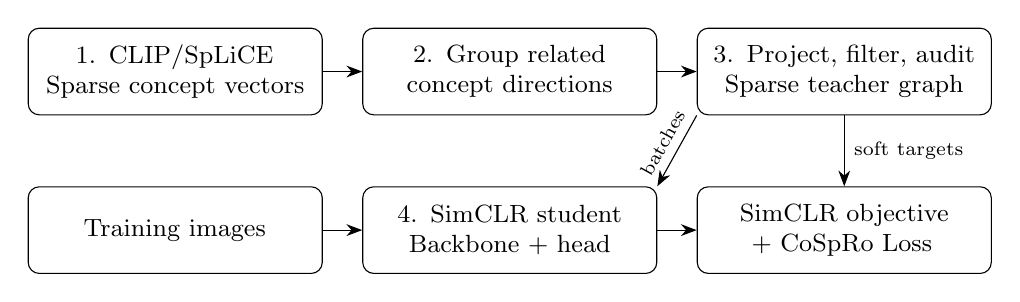
\begin{tikzpicture}[node distance=5mm and 5mm,
 box/.style={draw,rounded corners,align=center,font=\small,minimum height=11mm,text width=35mm},
 >={Stealth[length=2mm]}]
\node[box] (teacher) {1. CLIP/SpLiCE\\Sparse concept vectors};
\node[box,right=of teacher] (groups) {2. Group related\\concept directions};
\node[box,right=of groups] (graph) {3. Project, filter, audit\\Sparse teacher graph};
\node[box,below=9mm of teacher] (views) {Training images};
\node[box,right=of views] (student) {4. SimCLR student\\Backbone + head};
\node[box,right=of student] (loss) {SimCLR objective\\+ CoSpRo Loss};
\draw[->] (teacher)--(groups); \draw[->] (groups)--(graph);
\draw[->] (views)--(student); \draw[->] (student)--(loss);
\draw[->] (graph)--node[right,font=\scriptsize]{soft targets}(loss);
\draw[->] (graph.south west)--node[above,sloped,font=\scriptsize]{batches}(student.north east);
\end{tikzpicture}
\caption{The four-stage pipeline. Training images enter both the frozen teacher branch and the student branch. Graph construction and SSL use no target or group annotations. At inference the teacher, graph and SSL heads are discarded; a supervised linear probe evaluates the frozen student backbone.}
\label{fig:architecture}
\end{figure}

\subsection{Stage 1: SpLiCE concept representation}
 SpLiCE provides a sparse vector whose non-negative coordinates measure contributions of CLIP text directions to an image embedding. These coordinates let us test whether removing particular semantic information reveals a useful relation, without first annotating which concepts are spurious.

Given an image $x_i$, frozen CLIP produces an embedding $z_i$. We center and normalize it using the fixed SpLiCE mean $\mu$. With a row-normalized text dictionary $D\in\mathbb{R}^{K\times d}$, positive sparse regression gives
\begin{equation}
 u_i=\operatorname{norm}(z_i-\mu),\qquad
 c_i\in\arg\min_{c\geq0}\|u_i-D^\top c\|_2^2+\lambda_1\|c\|_1.
\end{equation}
All vectors are columns and \(\operatorname{norm}(v)=v/\lVert v\rVert_2\). Obtained concept decomposition $c_i$ of image $x_i$ can be read directly as a set of active concept coordinates. For example, if the dictionary contains the concepts \emph{grass}, \emph{cow} and \emph{alien}, one image might yield
\[
c_i =
0.72\,e_{\text{grass}}
+ 0.41\,e_{\text{cow}}
+ 0.18\,e_{\text{alien}},
\]
with most remaining coordinates equal to zero, where $e_k$ denotes the
coordinate associated with concept $k$. 

\subsection{Stage 2: Concept grouping}
Related words from dictionary D may describe overlapping semantic information (e.g. forest, jungle, trees). Removing only one direction can leave that information in another, so we allow related coordinates to form a joint subspace. We first exclude concepts that occur too rarely or almost everywhere in the training dataset, since they do not provide any useful semantic information, that would make other images closer to each other. Morphological variants of the same concept are joined directly (e.g., \emph{apple} and \emph{apples}).  For all other concept pairs $(k,l)$, we compute their text-direction similarity

\begin{equation}
    s^{\mathrm{text}}_{k\ell} = \cos(d_k,d_\ell)
\end{equation}  

and their activation similarity
\begin{equation}
  s^{\mathrm{act}}_{k\ell} = \cos(C_{:k},C_{:\ell}),  
\end{equation}

where $d_k$ is the dictionary direction of concept $k$ and $C_{:k}=(c_{1k},\ldots,c_{Nk})^\top$ collects its activations across all training images. Concepts are linked only when both similarities exceed their respective thresholds. Connected components of these links form concept groups, which can still consist of a single concept (singleton groups) if no other concept satisfy above mentioned requirements.

For each constructed concept group $G$, an SVD of its dictionary directions gives an orthonormal basis $Q_G$ for their span. Its image-level activation is $A_i^G=\sum_{k\in G}c_{ik}$. Each group is now represented by a subspace $Q_G$, describing \emph{what} semantic information it contains and an activation $A_i^G$, describing \emph{how strongly} that information is present in image $x_i$. Exact thresholds and numerical tolerances are given in Appendix~\ref{app:provenance}.

\subsection{Stage 3: Teacher-graph construction}
% A directed edge $i\!\to\!j$ means that image $j$ became a candidate neighbour of image $i$ after a concept group was removed, with increased similarity, contrasting group activation and agreement in the remaining concepts. Its weight measures this evidence. It does not certify that the pair has the same target or differs only in background.

\paragraph{Reveal and filter candidate relations.}
For each group $G$, we project the full centered embeddings outside its span:
\begin{equation}
 u_i^{-G}=\operatorname{norm}(u_i-Q_GQ_G^\top u_i)
\end{equation}

where $u_i^{-G}$ denotes normalized embedding of image $x_i$ after removing the component lying in subspace $G$. The gain
\begin{equation}
    \Delta_{ij}^{G} = \cos(u_i^{-G},u_j^{-G})-\cos(u_i,u_j)
\end{equation}
measures how much closer the two images become after removing group $G$. So $\Delta_{ij}^{G}>0$ indicates that directions associated with $G$ were partly responsible for separating $i$ and $j$ in the original representation.
We retain candidates with gain above a positive minimum threshold $\tau_D$.

However, the removed group should also be expressed differently in the two images. We therefore require a sufficiently large activation contrast $|A_i^G-A_j^G| > \tau_A $ between images $x_i$ and $x_j$. For example, if $G$ contains grass-related concepts, a candidate is more informative when these concepts are strongly active in one image but weakly active in the other.

A large gain can arise spuriously as well, since removing a subspace may make two otherwise unrelated images geometrically closer. We therefore check whether the concepts \emph{outside} $G$ are still alike. Let $c_i^{-G}$ denote the sparse decomposed vector of image $x_i$ with coordinates in $G$ removed. We measure residual concept agreement
\[
R_{ij}^{-G}
=
\cos(c_i^{-G},c_j^{-G})
\geq \tau_R,
\]
which receives stronger evidence when the remaining concepts match.

\paragraph{Audit groups and consolidate edges.}
Previous step evaluated individual candidate pairs. We now evaluate each concept group $G$ as a whole: a useful group should reveal a consistent set of relations, without being spuriously influenced by a few high-gain pairs caused by an arbitrary projection or accidental activation pattern.

We summarize the quality of group $G$ with a score $S(G)$ that rewards
four properties: large accepted gains $\Delta_{ij}^{G}$, broad anchor coverage, strong residual concept agreement $R_{ij}^{-G}$ and alignment between activation contrast and gain. A penalty downweights groups whose edges collapse onto a small number of destination images:

\begin{equation}
S(G)
=
\frac{
\operatorname{medianGain}(G)\,
\operatorname{coverage}(G)\,
\operatorname{agreement}(G)\,
\operatorname{alignment}(G)
}{
1+\operatorname{Gini}(G)+\operatorname{maxIndegree}(G)/N
}.
\end{equation}

A high group score is not sufficient by itself, because some score can arise
even when the removed subspace has no meaningful semantic role. We perform 2 tests where compare each group against synthetic null groups.

Equal-rank random subspaces test whether similar relation structure can be obtained by removing an arbitrary subspace of the same dimension. Shuffled activations test whether the observed activation--gain relationship survives when the concept activations are randomly reassigned across images.

The pooled null-score distribution defines a threshold $\tau_G$ at the chosen
quantile. A group is retained only if it has sufficient coverage and $S(G) > \tau_G$. Among the passing groups, a fixed cap keeps those with the largest excess above their null threshold.

We then convert the group's excess above the null threshold into a confidence factor:
\begin{equation}
 r_G=\min\!\left(1,\frac{\max(0,S(G)-\tau_G)}{\max(|S(G)|,\epsilon)}\right)
\end{equation}
This factor is close to zero for groups that barely exceed the null threshold and increases as the separation from the null becomes stronger. Each retained edge proposed by group $G$ is reweighted as
\[
\tilde e_{ij}^{G}=r_G * e_{ij}^{G}.
\]
Now same pairwise evidence contributes more when it comes from a well-calibrated group. 

After group-level calibration, we merge the surviving pairwise evidence across all retained groups. If multiple groups propose the same directed edge $i\rightarrow j$, we keep the strongest evidence. To keep the teacher graph sparse, we retain only the strongest outgoing edges for each anchor and impose a maximum destination indegree. The latter prevents a small number of images from becoming universal hubs.
 
After pruning, the remaining outgoing evidence for anchor $i$ is normalized into a teacher distribution
\[
p_T(j\mid i) = \frac{\tilde e_{ij}} {\sum_k \tilde e_{ik}}.
\]
This distribution specifies which donor images the teacher prefers for anchor $i$.

We also keep the absolute confidence of the strongest surviving relation:
\[
q_i=\max_j \tilde e_{ij}, \qquad q_i\in[0,1].
\]
Obtained $p_T(\cdot\mid i)$ describes the relative preference over donors and $q_i$ measures how strongly the teacher trusts the anchor's relational signal.

The result of pretraining stage is a fixed sparse teacher graph. Each supported anchor image $x_i$ has a small set of donor images, normalized teacher probabilities, an anchor confidence and an attribution to the concept group that produced the retained relation. Unsupported anchors contribute no relational loss.

\subsection{Stage 4: Graph-guided SimCLR training}
Now, built teacher graph will influence training in two ways. First, it changes batch composition so that graph-related images are more likely to appear together. Second, it provides a relational target that tells the student how similarity should be distributed among these images.

The standard two-view SimCLR objective remains unchanged: the positive pair for image $x_i$ is still formed by two augmentations of the same image. Teacher neighbours are therefore not substituted for SimCLR positives. 

The implemented graph-aware sampler still visits every training image once per epoch.  And whenever possible it places one of the anchor's teacher neighbours in the same batch. This increases the number of batches in which a graph relation can be used by introduced objective.

For a batch $B$, we obtain a backbone's representation of image $x_i$ before it is being processed by a projection head:
\[
s_i=\operatorname{norm}[\operatorname{norm}(h_i^{(1)})+\operatorname{norm}(h_i^{(2)})]
\] 
Pairwise cosine similarities within the batch are converted into a student distribution:
\begin{equation}
 p_S^B(j\mid i)=\frac{\exp(s_i^\top s_j/\tau_S)}
 {\sum_{k\in B:k\ne i}\exp(s_i^\top s_k/\tau_S)}.
\end{equation}
For anchor $i$, this distribution describes how the student sees similarity across the other images in the current batch.

The teacher distribution $p_T(\cdot\mid i)$ is defined over the full graph, however the student can only compare images present in the batch. We need to restrict $p_T$ to only use teacher neighbours that occur in current batch $B$ and renormalize the remaining probabilities, yielding $p_T^B$. 

The idea of relational loss is simple. The teacher distribution acts as the fixed target and the KL term encourages the student's similarity distribution to reproduce its relative donor preferences. Let $B_S=\{i\in B:\text{at least one teacher donor of $i$ occurs in }B\}$. The loss is
\begin{equation}
\mathcal{L}_{\mathrm{CoSpRo}} =
\frac{1}{|B_S|}
\sum_{i\in B_S} q_i\ * D_{\mathrm{KL}}
\left(
p_T^B(\cdot\mid i) \;\|\; p_S^B(\cdot\mid i)
\right).
\end{equation}
with $\mathcal{L}_{\mathrm{CoSpRo}}=0$ when $B_S$ is empty. Complete training objective is
\begin{equation}
\mathcal{L} = \mathcal{L}_{\mathrm{SimCLR}} + \lambda\mathcal{L}_{\mathrm{CoSpRo}}
\end{equation}

\section{Experimental Protocol}
We evaluate on Waterbirds using its 4,795 training images to build a fixed, label-free teacher graph and pretrain a randomly initialized ResNet-18. All main runs use 500 epochs, batch size 128, the same augmentations and optimization schedule, four student seeds and a single fixed graph seed. The SimCLR and relational temperatures are 0.05 and 0.25 and KL maximum relational weight of 0.5 is used.

We compare ordinary SimCLR, CoSpRo and raw-CLIP graph samplers without KL and the corresponding graphs with CoSpRo loss. Frozen student features at epoch 500 are evaluated with the same logistic probe fitted on 224 group-balanced training examples. Group labels are used for this probe and evaluation. We report mean and sample standard deviation across student seeds, using held-out test results for the main comparison and validation results for the additional controls. Full graph, training, probe and provenance settings appear in Appendices~\ref{app:provenance} and \ref{app:graphmath}.

\section{Results}
\subsection{Matched Waterbirds comparison}
\begin{table}[htbp]
\centering
\caption{Waterbirds held-out test evaluation at SSL epoch 500, seeds 1--4. Both KL configurations use $\lambda=0.5$. Values are percentages (mean $\pm$ sample standard deviation).}
\begin{tabular}{lrr}
\toprule
Method & Avg. & WGA \\
\midrule
SimCLR & $51.97 \pm 2.00$ & $46.82 \pm 3.65$ \\
CoSpRo sampler only & $51.95 \pm 3.32$ & $46.83 \pm 1.29$ \\
Raw CLIP sampler only & $50.86 \pm 2.61$ & $45.88 \pm 5.98$ \\
Raw CLIP + KL & $52.64 \pm 2.39$ & $48.48 \pm 3.44$ \\
\textbf{CoSpRo + KL} & $\textbf{53.38} \pm \textbf{1.84}$ & $\textbf{50.64} \pm \textbf{1.97}$ \\
\bottomrule
\end{tabular}
\label{tab:main}
\end{table}

CoSpRo achieves higher mean WGA by 3.82 percentage points relative to SimCLR and 2.16 points relative to matched raw-CLIP supervision in the four-seed Waterbirds evaluation (Table~\ref{tab:main}). The corresponding average-accuracy differences are +1.41 and +0.74 points. The sampler-only comparisons support a contribution from the relational objective beyond graph-aware batching. These results provide positive empirical evidence of improved robustness under the evaluated protocol. Appendix~\ref{app:seedresults} reports every seed and all four groups. The value $\lambda=0.5$ was selected empirically.

\subsection{Do projected relations add value beyond concept similarity?}
The semantic-graph control finds nearest neighbours of normalized SpLiCE reconstructions, preserving CoSpRo's supported anchors, row budgets, weight profiles, confidence and maximum indegree. Both use graph-aware batching and the same KL settings. Direct transfer instead predicts the normalized reconstruction through a separate head with cosine loss, ordinary batches and auxiliary weight 0.1 (Appendix~\ref{app:direct}). These comparisons distinguish projected relations, ordinary semantic relations and direct feature prediction.

\begin{table}[htbp]
\centering
\caption{Waterbirds validation at epoch 500, seeds 1--4. Mean $\pm$ sample standard deviation in percent. These controls share the backbone, optimization and probing protocol}
\begin{tabular}{lrr}
\toprule
Method & Avg. & WGA \\
\midrule
SimCLR & $52.11\pm1.37$ & $45.54\pm1.71$ \\
Raw CLIP graph + KL & $51.54\pm2.07$ & $46.97\pm2.83$ \\
Semantic SpLiCE graph + KL & $53.23\pm2.33$ & $48.00\pm4.48$ \\
Direct SpLiCE reconstruction & $52.81\pm2.12$ & $46.61\pm4.45$ \\
CoSpRo + KL & $53.46\pm3.05$ & $50.00\pm3.23$ \\
\bottomrule
\end{tabular}
\label{tab:semantic}
\end{table}

Across all four seeds, CoSpRo has 1.99-point higher mean WGA than semantic neighbours (Table~\ref{tab:semantic}). The paired differences are $+7.25,-1.88,+1.60,+1.01$ points: the evidence favors projected relations on average, but the effect is heterogeneous and modest relative to seed variation. CoSpRo's mean exceeds direct transfer by 3.39 points, without establishing general superiority of relational over coordinate transfer. Appendix~\ref{app:validation} reports all endpoints; Appendix~\ref{app:lassl} includes the single completed LA-SSL adaptation.

\subsection{What do the retained relations capture?}
The waterbirds graph has 12 selected concept groups and 12,239 directed edges, covering 4,582 of 4,795 training images (95.56\%), with maximum indegree 10. The selected concepts include Bamboo, Great grey owl and Tawny owl. All selected groups are singletons, so these experiments do not establish a benefit from multi-concept grouping.

Post-hoc labels show both useful cross-context relations and target mismatches (Appendix~\ref{app:graphaudit}). For landbirds on water, same-target cross-background relations carry 59.22\% of CoSpRo's confidence-weighted graph mass versus 44.96\% for the raw graph. For waterbirds on land, the corresponding share barely changes (48.26\% versus 48.95\%), while wrong-target mass increases to 45.76\% from 39.73\%. These failures suggest that projection can't claim to simply remove spurious information, despite improving mean test WGA. Frozen-feature diagnostics confirm that the concept representation contains useful predictive information, but use different preprocessing and external pretraining; they are reported separately in Appendix~\ref{app:signal}.

\section{Limitations}
The study uses one dataset, one frozen graph seed and four student seeds; estimated gains may change with graph construction or training randomness. The 224-example group-balanced probe uses labels and group annotations, so only graph construction and SSL are label-free. Results for this probe regime do not establish performance with a larger supervised budget.

Concept directions can mix object and background information. Projection reflects associations in the learned representation, while null calibration provides a reference for evaluating them and leaves causal interpretation and multiple-testing control to separate analyses. Wrong-target graph edges and mixed per-group outcomes indicate that projection removes some unwanted signal while preserving other spurious information. Auxiliary linear background probes reach 90.91--91.66\% validation accuracy across the four CoSpRo seeds, so background information remains accessible.

The method depends on CLIP's external pretraining and vocabulary coverage; sparse reconstruction loses some CLIP information. Graph construction adds preprocessing cost, though the core student runs share a 500-epoch budget. The semantic-graph and direct-transfer controls are seed-sensitive and do not establish that projection or relational transfer is generally superior.

\begin{samepage}
\section{Conclusion}
CoSpRo uses concept-subspace projections to build a fixed teacher graph for label-free relational pretraining of a separate encoder. On Waterbirds, its four-seed mean test average and worst-group accuracies exceed those of SimCLR and matched raw-CLIP graph supervision. Validation controls weakly favor projected over semantic neighbours. The graph contains wrong-target edges, so the results support a protocol-specific robustness gain, which can be studied even further.
\end{samepage}

\begingroup
\footnotesize
\setlength{\bibsep}{4pt plus 1pt}
\begin{thebibliography}{99}
\bibitem[Arefin et~al.(2024)]{arefin2024cobalt}
M.~R.~Arefin, Y.~Zhang, A.~Baratin, F.~Locatello, I.~Rish, D.~Liu and K.~Kawaguchi.
Unsupervised Concept Discovery Mitigates Spurious Correlations.
\emph{ICML}, pp.~1672--1688, 2024.
\url{https://proceedings.mlr.press/v235/arefin24a.html}.
\bibitem[Bhalla et~al.(2024)]{bhalla2024splice}
U.~Bhalla, A.~Oesterling, S.~Srinivas, F.~P.~Calmon and H.~Lakkaraju.
Interpreting CLIP with Sparse Linear Concept Embeddings (SpLiCE).
\emph{NeurIPS}, 2024. \url{https://arxiv.org/abs/2402.10376}.
\bibitem[Chen et~al.(2020)]{chen2020simclr}
T.~Chen, S.~Kornblith, M.~Norouzi and G.~Hinton.
A Simple Framework for Contrastive Learning of Visual Representations.
\emph{ICML}, pp.~1597--1607, 2020.
\url{https://proceedings.mlr.press/v119/chen20j.html}.
\bibitem[Chuang et~al.(2020)]{chuang2020debiased}
C.-Y.~Chuang, J.~Robinson, Y.-C.~Lin, A.~Torralba and S.~Jegelka.
Debiased Contrastive Learning. \emph{NeurIPS}, 2020.
\url{https://arxiv.org/abs/2007.00224}.
\bibitem[Dwibedi et~al.(2021)]{dwibedi2021nnclr}
D.~Dwibedi, Y.~Aytar, J.~Tompson, P.~Sermanet and A.~Zisserman.
With a Little Help From My Friends: Nearest-Neighbor Contrastive Learning
of Visual Representations. \emph{ICCV}, pp.~9588--9597, 2021.
\url{https://arxiv.org/abs/2104.14548}.
\bibitem[Ghorbani et~al.(2019)]{ghorbani2019ace}
A.~Ghorbani, J.~Wexler, J.~Zou and B.~Kim.
Towards Automatic Concept-based Explanations. \emph{NeurIPS}, 2019.
\url{https://arxiv.org/abs/1902.03129}.
\bibitem[Huynh et~al.(2022)]{huynh2022false}
T.~Huynh, S.~Kornblith, M.~R.~Walter, M.~Maire and M.~Khademi.
Boosting Contrastive Self-Supervised Learning with False Negative Cancellation.
\emph{WACV}, 2022. \url{https://arxiv.org/abs/2011.11765}.
\bibitem[Kim et~al.(2018)]{kim2018tcav}
B.~Kim, M.~Wattenberg, J.~Gilmer, C.~Cai, J.~Wexler, F.~Vi\'egas and R.~Sayres.
Interpretability Beyond Feature Attribution: Quantitative Testing with Concept Activation Vectors (TCAV).
\emph{ICML}, pp.~2668--2677, 2018. \url{https://proceedings.mlr.press/v80/kim18d.html}.
\bibitem[Koh et~al.(2020)]{koh2020cbm}
P.~W.~Koh, T.~Nguyen, Y.~S.~Tang, S.~Mussmann, E.~Pierson, B.~Kim and P.~Liang.
Concept Bottleneck Models. \emph{ICML}, pp.~5338--5348, 2020.
\url{https://proceedings.mlr.press/v119/koh20a.html}.
\bibitem[Liu et~al.(2021)]{liu2021jtt}
E.~Z.~Liu, B.~Haghgoo, A.~S.~Chen, A.~Raghunathan, P.~W.~Koh,
S.~Sagawa, P.~Liang and C.~Finn.
Just Train Twice: Improving Group Robustness without Training Group Information.
\emph{ICML}, pp.~6781--6792, 2021.
\url{https://proceedings.mlr.press/v139/liu21f.html}.
\bibitem[Oikarinen et~al.(2023)]{oikarinen2023lfcbm}
T.~Oikarinen, S.~Das, L.~M.~Nguyen and T.-W.~Weng.
Label-Free Concept Bottleneck Models. \emph{ICLR}, 2023.
\url{https://arxiv.org/abs/2304.06129}.
\bibitem[Park et~al.(2019)]{park2019rkd}
W.~Park, D.~Kim, Y.~Lu and M.~Cho.
Relational Knowledge Distillation. \emph{CVPR}, pp.~3967--3976, 2019.
\url{https://arxiv.org/abs/1904.05068}.
\bibitem[Radford et~al.(2021)]{radford2021clip}
A.~Radford et~al.
Learning Transferable Visual Models From Natural Language Supervision.
\emph{ICML}, pp.~8748--8763, 2021.
\url{https://proceedings.mlr.press/v139/radford21a.html}.
\bibitem[Robinson et~al.(2021a)]{robinson2021hard}
J.~Robinson, C.-Y.~Chuang, S.~Sra and S.~Jegelka.
Contrastive Learning with Hard Negative Samples. \emph{ICLR}, 2021a.
\url{https://arxiv.org/abs/2010.04592}.
\bibitem[Robinson et~al.(2021b)]{robinson2021shortcut}
J.~Robinson, L.~Sun, K.~Yu, K.~Batmanghelich, S.~Jegelka and S.~Sra.
Can contrastive learning avoid shortcut solutions? \emph{NeurIPS}, pp.~4974--4986, 2021b.
\url{https://arxiv.org/abs/2106.11230}.
\bibitem[Sagawa et~al.(2020)]{sagawa2020groupdro}
S.~Sagawa, P.~W.~Koh, T.~B.~Hashimoto and P.~Liang.
Distributionally Robust Neural Networks for Group Shifts: On the Importance
of Regularization for Worst-Case Generalization.
\emph{ICLR}, 2020. \url{https://arxiv.org/abs/1911.08731}.
\bibitem[von K\"ugelgen et~al.(2021)]{vonkugelgen2021content}
J.~von K\"ugelgen, Y.~Sharma, L.~Gresele, W.~Brendel, B.~Sch\"olkopf, M.~Besserve and F.~Locatello.
Self-Supervised Learning with Data Augmentations Provably Isolates Content from Style.
\emph{NeurIPS}, 2021. \url{https://arxiv.org/abs/2106.04619}.
\bibitem[Yalavarthi et~al.(2026)]{yalavarthi2026dial}
B.~C.~Yalavarthi, N.~Ratha and V.~Govindaraju.
Label-Free Mitigation of Spurious Correlations in VLMs using Sparse Autoencoders.
\emph{ICLR}, 2026.
\href{https://proceedings.iclr.cc/paper_files/paper/2026/hash/359242d225d2fba218a85e147803f8b7-Abstract-Conference.html}{ICLR 2026 proceedings}.
\bibitem[Yuksekgonul et~al.(2023)]{yuksekgonul2023pcb}
M.~Yuksekgonul, M.~Wang and J.~Zou.
Post-hoc Concept Bottleneck Models. \emph{ICLR}, 2023.
\url{https://arxiv.org/abs/2205.15480}.
\bibitem[Zheng et~al.(2021)]{zheng2021ressl}
M.~Zheng, S.~You, F.~Wang, C.~Qian, C.~Zhang, X.~Wang and C.~Xu.
ReSSL: Relational Self-Supervised Learning with Weak Augmentation.
\emph{NeurIPS}, 2021. \url{https://arxiv.org/abs/2107.09282}.
\bibitem[Zhu et~al.(2023)]{zhu2023lassl}
W.~Zhu, S.~Liu, C.~Fernandez-Granda and N.~Razavian.
Making Self-supervised Learning Robust to Spurious Correlation via
Learning-speed Aware Sampling. \emph{arXiv:2311.16361}, 2023.
\url{https://arxiv.org/abs/2311.16361v2}.

\bibitem[El Banani et~al.(2023)]{elbanani2023language}
M.~El Banani, K.~Desai and J.~Johnson.
Learning Visual Representations via Language-Guided Sampling.
\emph{CVPR}, 2023. \url{https://arxiv.org/abs/2302.12248}.

\bibitem[Ghosh et~al.(2026)]{ghosh2026cabs}
A.~Ghosh et~al.
Concept-Aware Batch Sampling Improves Language-Image Pretraining.
\emph{CVPR}, pp.~3056--3068, 2026.
\url{https://openaccess.thecvf.com/content/CVPR2026/html/Ghosh_Concept-Aware_Batch_Sampling_Improves_Language-Image_Pretraining_CVPR_2026_paper.html}.

\bibitem[Sachidananda et~al.(2023)]{sachidananda2023gcbs}
V.~Sachidananda, Z.~Yang and C.~Zhu.
Global Selection of Contrastive Batches via Optimization on Sample
Permutations. \emph{ICML}, pp.~29542--29562, 2023.
\url{https://proceedings.mlr.press/v202/sachidananda23a.html}.

\bibitem[Thirukovalluru et~al.(2025)]{thirukovalluru2025b3}
R.~Thirukovalluru et~al.
Breaking the Batch Barrier (B3) of Contrastive Learning via Smart
Batch Mining. \emph{NeurIPS}, 2025.
\url{https://proceedings.neurips.cc/paper_files/paper/2025/hash/21aa6840fcaa0cc3a1d16bafede47a2f-Abstract-Conference.html}.

\bibitem[Yang et~al.(2023)]{yang2023batchsampler}
Z.~Yang, T.~Huang, M.~Ding, Y.~Dong, R.~Ying, Y.~Cen,
Y.~Geng and J.~Tang.
BatchSampler: Sampling Mini-Batches for Contrastive Learning in Vision,
Language, and Graphs. \emph{KDD}, 2023.
\url{https://doi.org/10.1145/3580305.3599263}.

\bibitem[Khosla et~al.(2020)]{khosla2020supcon}
P.~Khosla et~al.
Supervised Contrastive Learning. \emph{NeurIPS}, 2020.
\url{https://arxiv.org/abs/2004.11362}.


\end{thebibliography}
\endgroup

\clearpage
\appendix
\section{Frozen Audit Configuration}
\label{app:provenance}
\begin{table}[ht]
\centering
\begin{tabularx}{\linewidth}{lX}
\toprule
Component & Completed-control setting \\
\midrule
Concept frequency & $[0.01,0.95]$ \\
Grouping & Text cosine 0.80; coactivation cosine 0.35; minimum size 1 \\
Projected neighbours & 20 per image \\
Residual code cosine & At least 0.25 \\
Activation contrast & Positive-gain difference quantile 0.75 \\
Minimum gain / coverage & $10^{-4}$ / 0.01 \\
Null calibration & 32 trials per family; pooled quantile 0.95 \\
Group cap & 12 after the full audit \\
Teacher graph & Up to 3 outgoing edges; maximum indegree 10 \\
Graph seed & 0 and shared across student seeds \\
\bottomrule
\end{tabularx}
\end{table}

\section{Per-Seed and Per-Group Results}
\label{app:seedresults}
\begin{table}[htbp]
\centering\small
\setlength{\tabcolsep}{4pt}
\caption{Waterbirds held-out test evaluation at epoch 500; KL weight 0.5. Groups are in form $(y,a)$. Values are percentages.}
\begin{tabular}{lrrrrrrr}
\toprule
Method & Seed & Avg. & WGA & (0,0) & (0,1) & (1,0) & (1,1) \\
\midrule
SimCLR & 1 & 49.34 & 42.17 & 42.17 & 47.45 & 65.58 & 64.95 \\
SimCLR & 2 & 51.50 & 45.63 & 45.63 & 56.90 & 52.18 & 52.49 \\
SimCLR & 3 & 53.24 & 49.89 & 49.89 & 54.46 & 56.70 & 57.32 \\
SimCLR & 4 & 53.78 & 49.58 & 53.88 & 49.58 & 56.39 & 65.58 \\
\addlinespace
Raw CLIP sampler & 1 & 52.83 & 49.49 & 49.49 & 54.72 & 55.45 & 55.30 \\
Raw CLIP sampler & 2 & 49.43 & 45.59 & 46.78 & 45.59 & 56.70 & 64.95 \\
Raw CLIP sampler & 3 & 47.91 & 37.56 & 37.56 & 49.05 & 66.82 & 61.37 \\
Raw CLIP sampler & 4 & 53.28 & 50.86 & 51.62 & 50.86 & 57.48 & 63.40 \\
\addlinespace
CoSpRo sampler & 1 & 50.05 & 45.94 & 45.94 & 47.01 & 59.97 & 65.26 \\
CoSpRo sampler & 2 & 49.41 & 46.25 & 47.85 & 46.25 & 54.21 & 61.21 \\
CoSpRo sampler & 3 & 51.59 & 46.39 & 46.39 & 49.67 & 62.93 & 65.26 \\
CoSpRo sampler & 4 & 56.73 & 48.75 & 58.98 & 56.32 & 48.75 & 58.26 \\
\addlinespace
Raw CLIP + KL & 1 & 50.38 & 47.05 & 47.05 & 50.78 & 54.36 & 56.70 \\
Raw CLIP + KL & 2 & 52.14 & 47.27 & 51.75 & 47.27 & 57.63 & 65.11 \\
Raw CLIP + KL & 3 & 52.02 & 46.03 & 46.03 & 49.67 & 68.07 & 65.26 \\
Raw CLIP + KL & 4 & 56.01 & 53.57 & 53.57 & 57.56 & 55.92 & 59.19 \\
\addlinespace
CoSpRo + KL & 1 & 53.85 & 51.40 & 51.40 & 53.57 & 55.45 & 61.84 \\
CoSpRo + KL & 2 & 51.83 & 49.22 & 51.84 & 49.22 & 51.40 & 61.37 \\
CoSpRo + KL & 3 & 52.05 & 48.87 & 48.87 & 50.29 & 60.59 & 60.90 \\
CoSpRo + KL & 4 & 55.78 & 53.08 & 53.08 & 58.63 & 54.05 & 57.01 \\
\addlinespace
\bottomrule
\end{tabular}
\end{table}

\begin{table}[htbp]
\centering\small
\caption{Paired CoSpRo differences in percentage points at final epoch}
\begin{tabular}{rrrrrrr}
\toprule
& \multicolumn{2}{c}{vs. SimCLR} & \multicolumn{2}{c}{vs. own sampler} & \multicolumn{2}{c}{vs. raw CLIP + KL} \\
Seed & $\Delta$Avg. & $\Delta$WGA & $\Delta$Avg. & $\Delta$WGA & $\Delta$Avg. & $\Delta$WGA \\
\midrule
1 & +4.51 & +9.22 & +3.80 & +5.45 & +3.47 & +4.35 \\
2 & +0.33 & +3.59 & +2.42 & +2.97 & -0.31 & +1.95 \\
3 & -1.19 & -1.02 & +0.47 & +2.48 & +0.03 & +2.84 \\
4 & +2.00 & +3.50 & -0.95 & +4.33 & -0.22 & -0.49 \\
\midrule
Mean & +1.41 & +3.82 & +1.43 & +3.81 & +0.74 & +2.16 \\
\bottomrule
\end{tabular}
\end{table}

\section{Graph and Loss Details}\label{app:graphmath}

\paragraph{Projection and group-score details.}
The SVD basis retains singular values satisfying
\[
\sigma > 10^{-6}\max(\sigma_{\max},1).
\]
Projected embeddings with norm at most $10^{-12}$ are rejected; zero-norm residual codes receive similarity zero. In $S(G)$, median gain, coverage, mean residual agreement and destination indegrees use accepted edges. Alignment is the correlation of $|A_i^G-A_j^G|$ with $\Delta_{ij}^G$ among positive-gain candidates before the residual gate, clipped to $[0,1]$. Neighbor concentration is measured using the Gini coefficient of destination indegrees and the maximum indegree.

\paragraph{Null calibration and graph pruning.}
For each group, 32 equal-rank Gaussian-subspace trials recompute projected neighbours and 32 activation-shuffle trials retain the original geometry and residual agreement. Both use the observed candidate-selection and scoring procedure. The pooled score $0.95$ quantile defines $\tau_G$; passing groups are ranked by $S(G)-\tau_G$ and capped at 12.

Duplicate directed edges keep the strongest evidence, followed by caps of three outgoing edges per anchor and ten incoming edges per destination. Of 504 audited groups (503 singletons and one pair), 441 (87.5\%) exceed their null threshold and 12 survive the cap.

\paragraph{Implemented training objective.}
For normalized projection-head views $v_a$ in batch $B$, the implemented SimCLR term is
\begin{equation}
\mathcal{L}_{\mathrm{SimCLR}} = -\frac{\tau_C}{0.07} \frac{1}{2|B|}
\sum_a \log
\frac{
    \exp(v_a^\top v_{a^+}/\tau_C)
}{
    \sum_{b\neq a}\exp(v_a^\top v_b/\tau_C)
}.
\end{equation}
Here $a^+$ is the other view of the same image. The factor $\tau_C/0.07$ follows the SupCon implementation's temperature scaling \citep{khosla2020supcon}.

The relational softmax uses backbone representations and masks the anchor ID. Only donors present in the batch enter the restricted teacher distribution, with zero teacher mass on other batch members, meaning anchors without a donor contribute no relational loss. The relational weight starts after epoch 10, rises over ten epochs to $\lambda_{\max}=0.5$ and stays there through epoch 500. This value was chosen in a preliminary development comparison. An empty graph falls back to SimCLR, but graph-control experiments require nonempty graphs.

\section{Post-hoc Graph Audit}\label{app:graphaudit}
The selected graph has 12 concept groups and 12,239 directed edges, supporting 4,582/4,795 anchors (95.56\% coverage); maximum indegree is 10 and indegree Gini is 0.573. Post-hoc labels show uneven relation quality: among the 56 training waterbirds on land, CoSpRo has 48.26\% same-target cross-background mass and 45.76\% wrong-target mass, versus 48.95\% and 39.73\% for the raw graph. Labels were excluded from construction.

\begin{table}[htbp]
\centering\small
\caption{Post-hoc composition of confidence-weighted graph mass, in percent within each source group $(y,a)$. Cross-bg. denotes same-target, different-background edges; wrong-target includes both backgrounds. Annotations are used only after graph construction.}
\begin{tabular}{lrrrr}
\toprule
& \multicolumn{2}{c}{Raw CLIP} & \multicolumn{2}{c}{CoSpRo} \\
Source group & Cross-bg. & Wrong-target & Cross-bg. & Wrong-target \\
\midrule
$(0,0)$ & 0.57 & 0.92 & 1.18 & 1.31 \\
$(0,1)$ & 44.96 & 25.60 & 59.22 & 25.11 \\
$(1,0)$ & 48.95 & 39.73 & 48.26 & 45.76 \\
$(1,1)$ & 1.25 & 8.66 & 2.51 & 9.77 \\
\bottomrule
\end{tabular}
\label{tab:graph}
\end{table}

\section{Frozen Representation Diagnostics}\label{app:signal}
\begin{table}[H]
\centering
\caption{Frozen-feature diagnostic with the same 224 probe-training IDs and L2 coefficient 0.001. Values are validation percentages. These representations use deterministic diagnostic preprocessing and external pretraining where applicable; they are not matched SSL student runs.}
\begin{tabular}{lrrr}
\toprule
Representation & Dimension & Avg. & WGA \\
\midrule
Centered OpenCLIP & 512 & 79.82 & 75.37 \\
SpLiCE codes & 20931 & 68.31 & 64.16 \\
SpLiCE reconstruction & 512 & 77.98 & 72.75 \\
Random ResNet-18 & 512 & 45.87 & 40.04 \\
ImageNet ResNet-18 & 512 & 78.98 & 76.23 \\
\bottomrule
\end{tabular}
\label{tab:signal}
\end{table}

The SpLiCE reconstruction yields 77.98\% Avg. and 72.75\% WGA on this diagnostic. All five probes fit the 224 training examples perfectly, including the random encoder, so training accuracy alone does not show generalization at this sample size.

\section{Direct Transfer and Validation Endpoints}
\label{app:direct}
\label{app:validation}

For direct reconstruction transfer, a separate head $g_\psi$ predicts the
unit-normalized frozen SpLiCE reconstruction $t_i$ from each student view:
\begin{equation}
 \mathcal{L}_{\mathrm{transfer}}=
 \frac{1}{2|B_V|}\sum_{i\in B_V}\sum_{v=1}^{2}
 \left[1-\cos\!\left(g_\psi(f_\theta(x_i^{(v)})),t_i\right)\right].
\end{equation}
Here $B_V$ contains valid target rows. Training minimizes
$\mathcal{L}_{\mathrm{SimCLR}}+\alpha(t)\mathcal{L}_{\mathrm{transfer}}$
with ordinary batches and SimCLR temperature 0.05. The transfer weight starts
after epoch 10, rises to 0.1 over the next ten epochs and remains there
through epoch 500.

Table~\ref{tab:semantic} gives four-seed means. The endpoints below show
their seed variation under the same probe protocol. They are validation
results and should not be compared numerically with the held-out test
results in Table~\ref{tab:main}.

\begin{table}[htbp]
\centering\small
\caption{Validation Avg./WGA percentages at SSL epoch 500.}
\begin{tabular}{lrrrr}
\toprule
Method & Seed 1 & Seed 2 & Seed 3 & Seed 4 \\
\midrule
SimCLR & 50.29 / 44.54 & 51.96 / 43.68 & 52.63 / 47.32 & 53.54 / 46.62 \\
Raw CLIP + KL & 50.38 / 44.33 & 49.46 / 46.57 & 52.21 / 46.04 & 54.13 / 50.96 \\
Semantic SpLiCE & 54.05 / 44.36 & 54.13 / 51.88 & 49.79 / 43.90 & 54.96 / 51.88 \\
Direct reconstruction & 54.71 / 50.75 & 49.79 / 43.47 & 53.54 / 50.11 & 53.21 / 42.11 \\
CoSpRo + KL & 55.80 / 51.61 & 53.29 / 50.00 & 49.21 / 45.49 & 55.55 / 52.89 \\
\bottomrule
\end{tabular}
\end{table}

\section{LA-SSL Adaptation}\label{app:lassl}
We implement the learning-speed-aware sampling rule of \citet{zhu2023lassl} within the same ResNet-18, 500-epoch, batch-size-128 SimCLR and linear-probe protocol. Learning-speed estimates use exponentiated two-view projection similarity and an exponential moving average. The adaptation uses EMA coefficient 0.1, sampling scale 10 and quantile 0.1, updating every two epochs after a ten-epoch warm-up (first update at epoch 12).

\begin{table}[H]
\centering\small
\caption{LA-SSL validation results at SSL epoch 500. Groups follow $(y,a) = 00, 01, 10, 11$. Mean and sample standard deviation are across seeds.}
\begin{tabular}{lrrrrrr}
\toprule
Seed & Avg. & WGA & 00 & 01 & 10 & 11 \\
\midrule
1 & 50.38 & 45.61 & 45.61 & 50.43 & 53.38 & 63.91 \\
2 & 52.13 & 46.68 & 46.68 & 55.15 & 54.89 & 57.89 \\
3 & 51.79 & 45.18 & 45.18 & 54.94 & 60.15 & 55.64 \\
4 & 53.38 & 47.54 & 47.54 & 55.15 & 53.38 & 67.67 \\
\midrule
Mean $\pm$ SD & $51.92\pm1.23$ & $46.25\pm1.06$ & & & & \\
\bottomrule
\end{tabular}
\label{tab:lassl}
\end{table}

All four probes converged at epoch 500 and group 00 is the worst group in every seed. Relative to matched SimCLR, LA-SSL's four-seed mean changes Avg./WGA by $-0.19/+0.71$ points. Relative to CoSpRo, it is lower by 1.54 Avg. points and 3.74 WGA points.

\end{document}
